\documentclass{beamer}

%Include Packages
\usepackage{amsmath}
\usepackage{amssymb}
\usepackage[normalem]{ulem}		%For underline
\usepackage{graphicx}
\usepackage{tikz}

%\usepackage{beamerthemesplit}
\usetheme{Warsaw}
%\usecolortheme{dolphin}
\logo{
\includegraphics[height=0.6cm]{logo}}

%Top Matter
\title[]{A Monte Carlo Study of the Classical, Isotropic, 3D Heisenberg Model}
\subtitle{Numerical Studies of Stochastic Spin Systems}
\author[]{Michael Conroy\\
  PHY 471 Capstone Project \\
  Spring 2014 \\
  Professor: Dr. Matthew Enjalran}
\date{May 2, 2014}

\begin{document}
	%Title Frame
	\begin{frame}
	%\frametitle{}
	\titlepage
	\end{frame}

	%Table of Contents Frame
	\begin{frame}
		\frametitle{Table of Contents}
		\tableofcontents
	\end{frame}

	\section{Introduction}
	
	\subsection{Goal}
  \begin{frame}
    \frametitle{Goal and Purpose}
    	\begin{itemize}
    		\item Simulate the classical, isotropic, 3D Heisenberg Model on the simple cubic lattice
    		\item Utilize the Monte Carlo method with the Metropolis Algorithm
    		\item Compare simulation data to literature data
    		\item Explore numerical analysis approach to the simulation
    	\end{itemize}
  \end{frame}
  
  \subsection{Brief Overview}
  \subsubsection*{Heisenberg Model}
  \begin{frame}
    \frametitle{Heisenberg Model}
    	\begin{columns}[t]
    	\begin{column}[T]{5cm}
    		\begin{itemize}
    			\item Continuous spin model
    			\item Hamiltonian: \\
    						$\displaystyle H = -J\sum_{<ij>}^{N}\vec{S_i}\cdot\vec{S_j}$, \\ where $\displaystyle |\vec{S_i}| = 1$.
    			\item Applications    						
    		\end{itemize}
    	\end{column}
    	\begin{column}[T]{6cm}
    		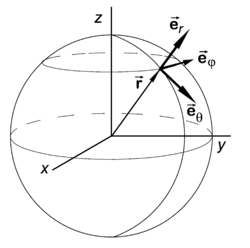
\includegraphics[scale=1.5]{spherical_unit_vector} 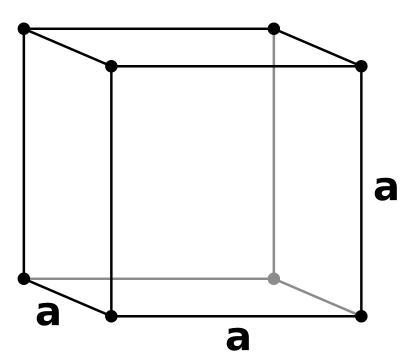
\includegraphics[scale=0.1]{sc} \\
    		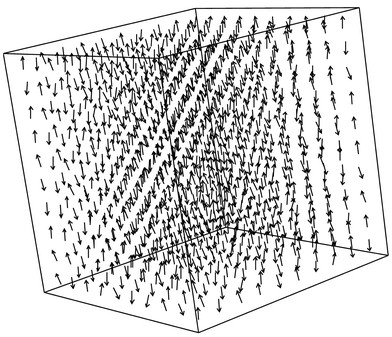
\includegraphics[scale=0.4]{lattice}
    	\end{column}
    	\end{columns}
  \end{frame}
  \subsubsection*{Magnetism and Magnetism in Statistical Mechanics}
  \begin{frame}
    \frametitle{Magnetism and Magnetism in Statistical Mechanics}
    	\begin{itemize}
    		\item Magnetic Domains \\
    					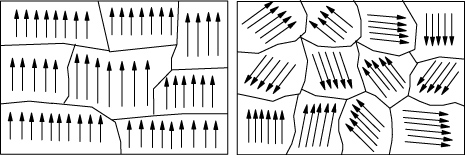
\includegraphics[scale=0.5]{domains}
    		\item Paramagnetism, ferromagnetism, and antiferromagnetism \\
    					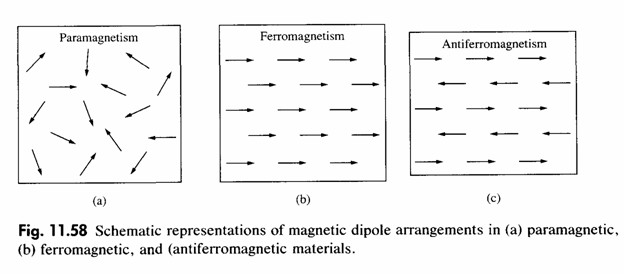
\includegraphics[scale=0.3]{ferro_para_anti}
    	\end{itemize}
  \end{frame}
  \subsubsection*{Phase Transitions}
  \begin{frame}
    \frametitle{Phase Transitions}
    	\begin{itemize}
    		\item Critical Temperature
    		\item Order Parameter
    	\end{itemize}
  \end{frame}
  \subsubsection*{Numerical Analysis}
  \begin{frame}
    \frametitle{Numerical Analysis}
    \begin{columns}[t]
    	\begin{column}[T]{4.7cm}
    		\begin{itemize}
    			\item No analytic solutions
    			\item Intractable problems
    			\item Monte Carlo simulations
    			\begin{itemize}
    				\item Importance sampling
    			\end{itemize}
    			\end{itemize}
    	\end{column}
    	\begin{column}[T]{7cm}
  			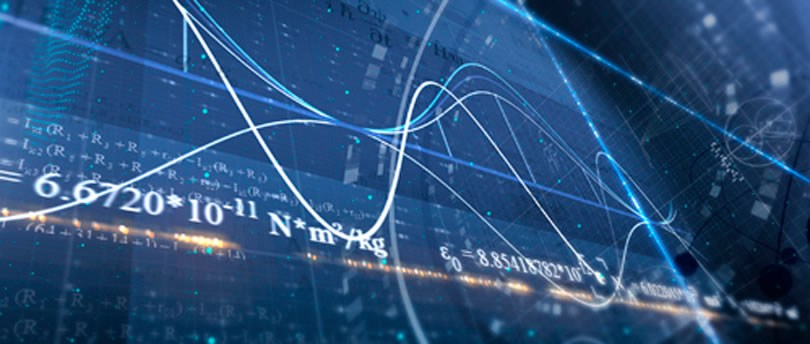
\includegraphics[scale=0.25]{numerical_analysis}
  		\end{column}
		\end{columns}	
  \end{frame}

	\section{Background and Theory}
	
	\subsection{Statistical Mechanics}
  \begin{frame}
    \frametitle{Statistical Mechanics}
    \framesubtitle{}
    \begin{itemize}
    	\item Canonical Ensemble
    	\item Boltzmann Distribution: $\displaystyle p_\mu = \frac{1}{Z(\beta)}e^{-\beta E(\mu)}$
    	\item Partition Function: $\displaystyle Z(\beta) = \sum_\mu e^{-\beta E(\mu)}$
    	\item Most macroscopic thermodynamic variables of a system can be expressed by the partition function or its derivatives!
    	\item For example, energy, specific heat, entropy, free energy...
    \end{itemize}
  \end{frame}
  \subsection{The Heisenberg Model}
  \begin{frame}
    \frametitle{Calculating the Physical Quantities}
    \framesubtitle{}
    \begin{itemize}
    	\item How do we calculate the required physical quantitites of the Heisenberg Model?
      \item Energy and specific heat:\\
      			$\displaystyle E = -J\sum_{<ij>}^{N}\vec{S_i}\cdot\vec{S_j}$ \\
      			$\displaystyle C = k\beta^2(\left< E^2 \right> - \left< E \right>^2)$ \\
    	\item Magnetization: \\
    				$\displaystyle m = \sqrt{M_x^2 + M_y^2 + M_z^2}$,\\
    				 where $\displaystyle M_\alpha = \frac{1}{N}\sum_i{\vec{S_{i\alpha}}}$
    	
    \end{itemize}
  \end{frame}
  \subsection{Monte Carlo Method}
  \begin{frame}
    \frametitle{Background and Theory}
    \framesubtitle{}
    \begin{itemize}
    	\item Numerical Analysis
    	\begin{itemize}
    		\item No analytic solution or intractable
    	\end{itemize}
    	\item Pseudo-random number generation
    	\item Monte Carlo Simulation
    	\begin{itemize}
    		\item Estimator
    		\item Importance Sampling
    		\begin{itemize}
    			\item Markov Processes
    			\item Ergodicity
    			\item Detailed Balance
    		\end{itemize}
    		\item Acceptance Ratio
    	\end{itemize}
    \end{itemize}
  \end{frame}

	\section{Method}
	\subsection{Implementation}
	\subsubsection*{Software}
  \begin{frame}
    \frametitle{Implementation}
    \framesubtitle{Software}
    \begin{columns}[t]
    	\begin{column}[T]{5cm}
    		\begin{itemize}
    			\item KISS: "Keep It Simple Stupid"
    			\item Functional Approach in C
    			\item 3D and 4D Pseudo-arrays of Pointers
    			\item GNU GCC Compiler, Code::Blocks IDE
   			\end{itemize}
      \end{column}
    	\begin{column}[T]{6.5cm}
    		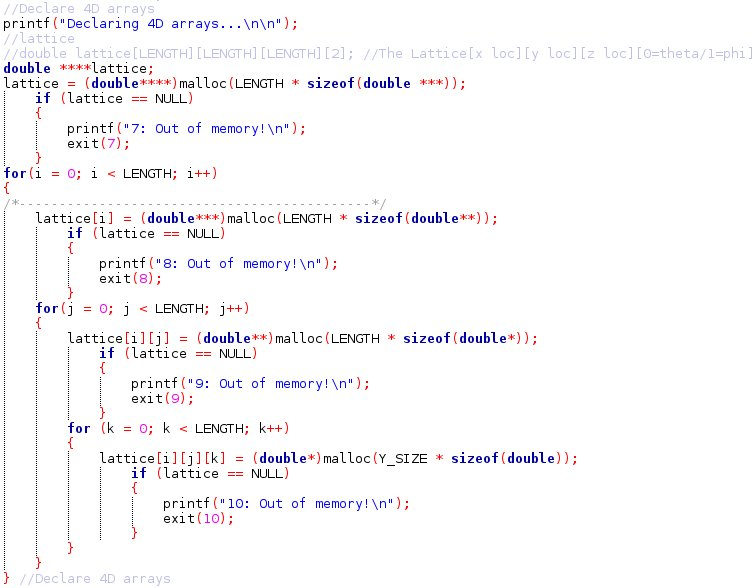
\includegraphics[scale=0.35]{code1}
    	\end{column}
    \end{columns}
  \end{frame}
  \subsubsection*{Hardware}
  \begin{frame}
    \frametitle{Implementation}
    \framesubtitle{Hardware}
    \begin{itemize}
    	\item Workstation\\
    				Lenovo IdeaPad Y580 \\
    				Intel i7-3630QM,  8-thread, 3.4 GHz (max, single core) \\
    				16 GB ram, 256 GB SSD \\
    				GeForce GTX 660M (overclocked to 1 GHz) \\
    				Fedora 20 Linux, Scientific Spin
    	\item Simulation Machines\\
    				Custom Built PCs \\
    				AMD Opteron 6212, 16-thread, 3.2 GHz (max, $\le$ 4 core) \\
    				32GB ram, Fedora and Ubuntu Linux
    \end{itemize}
  \end{frame}
    
  \section{Results and Discussion}
  \subsection{Data Plots}
  \begin{frame}
    \frametitle{Data Plots}
    \framesubtitle{Energy}
  \end{frame}
  \begin{frame}
  	\frametitle{Data Plots}
    \framesubtitle{Magnetization}
  \end{frame}
  %Specific Heat
  \begin{frame}
  	\frametitle{Data Plots}
    \framesubtitle{Specific Heat}
  \end{frame}
  %Susceptibility
  \begin{frame}
  	\frametitle{Data Plots}
    \framesubtitle{Magnetic Susceptibility}
    \begin{itemize}
    	\item \textbf{Susceptibility calculation not straightforward due to rotational invariance in 3D Heisenberg Model!}
    \end{itemize}
  \end{frame}
  
  \section{Conclusion}
  \subsection*{Conclusion}
  \begin{frame}
    \frametitle{Conclusion}
    \begin{itemize}
      \item Data matches predicted behavior
      \item Phase transition at critical temperature of $T_c \approx 1.45 K$
    	\item Susceptibility not as straightforward to calculate as in the Ising Model
    	\item Acceptance ratio oddity
    	\item Programmatic concerns
    	\begin{itemize}
    		\item Code in Fortran for readability, debugging, and intrinsic functions (but be careful!)
    		\item Fix arrays and possibly implement structures
    		\item Improve simulation run time! Optimize code!
    	\end{itemize}
    \end{itemize}
  \end{frame}
  
  \subsection*{Future Work}
  %Frame 10
  \begin{frame}
    \frametitle{Next Steps and Future Work}
    \begin{itemize}
      \item Code improvements
    	\item Susceptibility
    	\begin{itemize}
    		\item Correlation function calculation    	
    	\end{itemize}
    	\item Spin dynamics
    	\item Magnetic frustration and other lattices
    	\item Possible project: LED Cube visualization of 3D Ising model phase change
    \end{itemize}
  \end{frame}

\end{document}
